\documentclass{article}
\usepackage[utf8]{inputenc}
\usepackage[T1]{fontenc}
\usepackage{graphicx}
\usepackage{amsmath}
\usepackage{wrapfig}
\usepackage[top=1in, bottom=1.25in, left=1.1in, right=1.1in]{geometry}

\title{Reporte - Actividad 10: Teoría del Caos y el Mapeo Logístico}
\author{García Monge Itzel Alexia}
\date{16 de Mayo, 2018}


\begin{document}
\maketitle

\section{Introducción}
Para esta actividad se recurrió al uso de wxMaxima para graficar la Teoría del Caos y su respectivo mapeo logístico. Se trataron de recrear de la manera más precisas las gráficas encontradas en el trabajo \textit{Chaos Theory and the Logistic Map} por Geoff Boeing, quién uso \textit{Python} cómo su lenguaje de programación de elección.

\section{Teoría del Caos y Mapeo Logístico}
La \textit{Teoría del Caos} es una rama de las matemáticas que trata sistemas dinámicos no lineales. Los sistemas caóticos son simplemente un subtipo de sistemas dinámicos no lineales, conteniendo muy pocas partes que interactúan. Estas partes pueden seguir reglas simples, pero los sistemas tienen una dependencia tan extremadamente sensible que al pasar el tiempo pueden producir un comportamiento totalmente impredecible y divergente.

\section{Mapeo Logístico}
Se llama mapeo logístico porque el mapea el valor de la población en cualquier tiempo específico a su valor del siguiente tiempo específico. Podemos mostrar como funciona el mapeo logístico usando un modelo que se basa comúnmente en una curva S de función logística que muestra como una población crece lentamente, luego rápidamente, antes de disminuir al acercarse a su capacidad de carga. En el mapeo logístico se usa una ecuación diferencial no linear para mirar el tiempo como pasos discretos.

Se expresa con la ecuación:
$x_{t+1}= rx_t(1-x_t)$

la cual define las reglas, o dinámicas, de nuestro sistema, siendo \textit{X} el representante de la población a cualquier tiempo dado \textit{t}, y \textit{r} representando la tasa de crecimiento. Si la tasa de crecimiento es muy baja, la población terminará muriendo y caerán en extinción, en cambio, si la tasa de crecimiento sube se puede alcanzar un valor estable o que fluctue a través de una serie de booms en la población.

Aunque a primera vista parece ser una ecuación simple, dependiendo del parámetro en la tasa de crecimiento se obtiene caos.


\section{Sistema de Comportamiento y Atractores}
Observemos los siguientes gráficos de línea para 20 generaciones:

	\begin{center}
    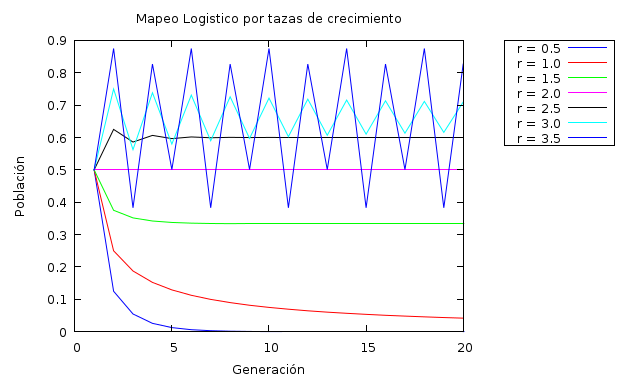
\includegraphics[height=6cm]{graf1.png}
    \end{center}


Se puede apreciar fácilmente la población cambia al pasar el tiempo cuando se le dan diferentes tasas de crecimiento. La gráfica azul representa un crecimiento con tasa del 0.5, haciendo que baje a cero de manera casi inmediata, es decir, la población muere. En camio, la gráfica cyan representa una tasa del 2.0 y se mantiene estable en un nivel de población de 0.5. Por último, las gráficas verdaderamente interesante son las gráficas con tasa de 3.0 y 3.5, ya que mientras parece que la gráfica de 3.0 está convergiendo lentamente hacia un valor estable, la gráfica de 3.5 parece estar rebotando.

Para cada tasa de crecimiento menor que 1.0 el sistema colapsa a cero, para tasas de crecimiento mayor entre 1.0 y 3.0 el sistema se mantiene en un nivel de población estable. Pero para cada tasa de crecimiento de mayores a 3.0en adelante nunca se mantiene en un punto o ciclo límite-obtenemos caos.

Un atractor es uno, o un conjunto de, valores que el sistema establece después de cierto periodo de tiempo. Cuando ajustamos el parámetro de su tasa a más de 3.5, obtenemos caos. Un sistema caótico tiene un extraño atractor por el cual el sistema oscila permanentemente, nunca golpeando el mismo punto más de una vez y su estructura tiene forma fractal. Esto quiere decir que el mismo patrón existe en casa escala sin importar cuanto lo acerques a detalle.

\section{Bifurcaciones y el Camino al Caos}
Para una mejor apreciación, corramos un mapeo logístico para 200 generaciones con 1,000 tasas de crecimiento entre 0.0 y 4.0. Como esta vez contamos con más tasas de crecimiento, se utiliza un diagrama de bifurcación para observar los resultados.


	\begin{figure}[h!]
    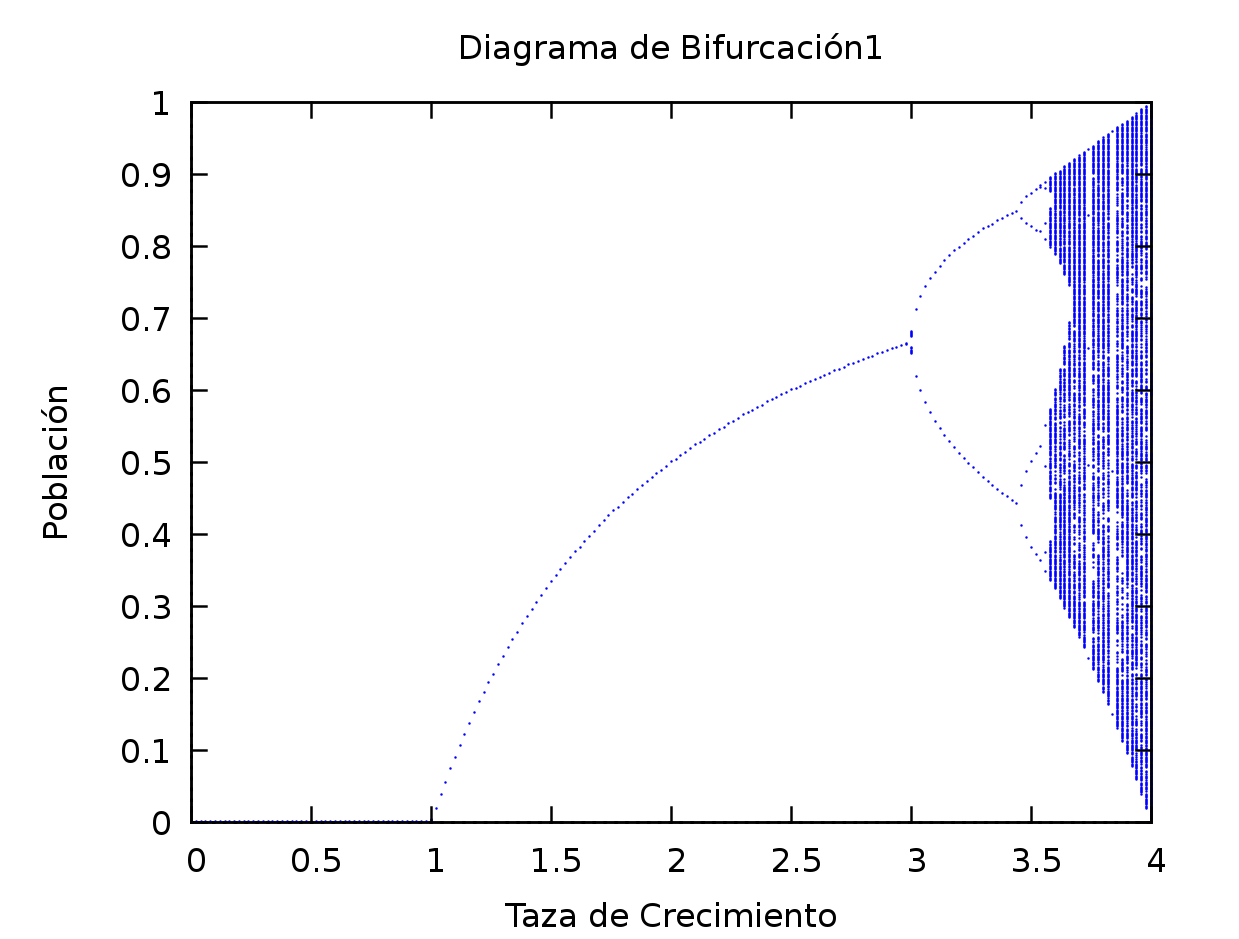
\includegraphics[height=6cm]{graf2.png}
    \centering
    \end{figure}

Pensemos en el diagrama siguiente como 1,000 rodajas verticales, cada una correspondiendo a una de los parámetros para las 1,000 tasas de crecimiento. Para cada rodaja, el modelo se corre 200 veces para luego tirar los primeros 100 valores, teniendo finalmente 100 generaciones por tasa de crecimiento. En pocas palabras, la rodaja sobre cada tasa de crecimiento es la atractor de la tasa de crecimiento misma. 

Para poder entender el nombre \textit{diagrama de bifurcación}, observemos con más detalle el diagrama generado.


	\begin{figure}[h!]
    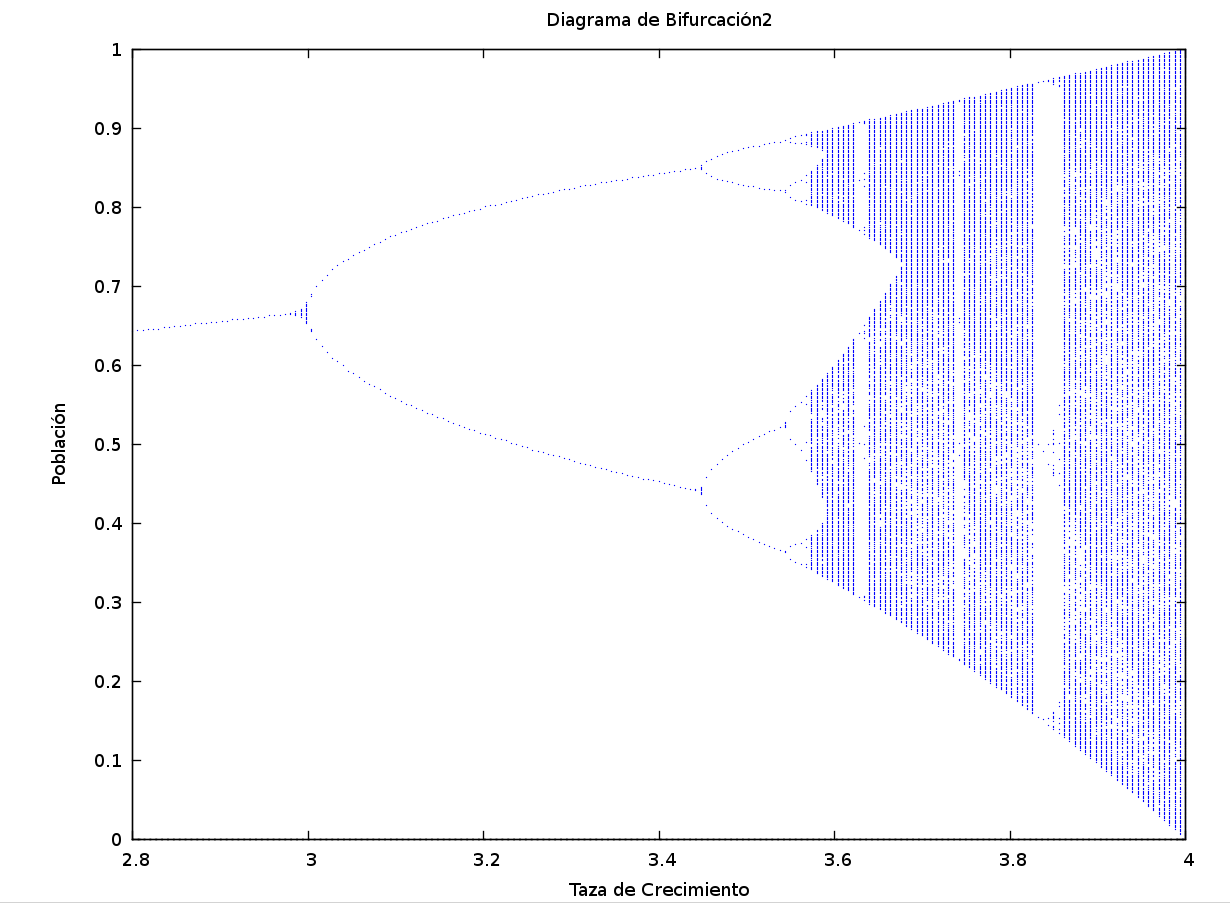
\includegraphics[height=6cm]{graf3.png}
    \centering
    \end{figure}

Podemos apreciar como al principio los posibles valores se separan en dos cuando la tasa de crecimiento alcanza el 3.0, luego lo hace nuevamente en cuatro separaciones al alcanzar 3.4, para finalmente separarse en 8 cuando se obtiene el parámetro 3.5. Estas separaciones reciben el nombre de bifurcaciones.

\section{El Comienzo del Caos}
Cuando los valores rebasan la tasa de crecimiento del 3.6, las bifuraciones van aumentando hasta que eventualmente pueden caer en cualquier valor poblacional, conocido comúnmente como el periodo de duplicación del caos. Conforme se ajusta el parámetro de la tasa de crecimiento a valores poblacionales más altos, el mapeo logístico oscilará entre dos, luego cuatro, luego ocho, y así seguirá hasta llegar a 3.9, donde habrá bifurcado tantas veces que el sistema brinca-aparentemente de manera aleatoria-entre valores poblacionales.

Aunque los valores que se obtienen parecen ser aleatorios, en realidad no lo son, siguen un modelo con reglas deterministas simples pero parecen producir aleatoriedad.

Demos aún más detalle a las gráficas anteriores cuando sus valores están entre 3.7 y 3.9:

	\begin{figure}[h!]
    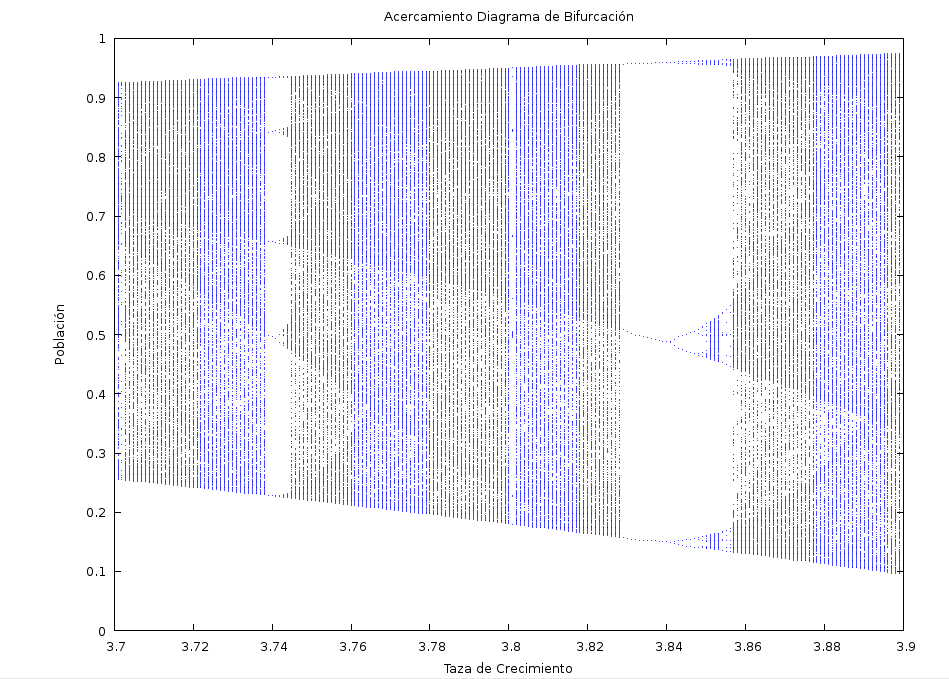
\includegraphics[height=6cm]{graf4.png}
    \centering
    \end{figure}

En está gráfica se puede lograr apreciar la belleza del caos. Fuera de todo el ruido emerge, entre cada lado de donde el sistema se comporta distinto, un patrón arremolinado de forma extraña. Entre los parámetros de la tasa de crecimiento de 3.82 y 3.84, el sistema se mueve del caos hacia el orden, para luego bifurcar nuevamente y regresar al caos cuando su tasa de crecimiento llega a 3.86.

\section{Fractales y Atractores Extraños}
Si dejamos de ver tan detalladamente el diagrama de bifurcación y nos alejamos un poco, encontramos que la estructura que observamos a nivel micro también puede verse a nivel macro. Incluso si hacemos un acercamiento infinito, seguiremos observando la misma estructura. Esto ocurre debido a los extraños atractores que tiene un sistema caótico, así como su estructura, la cual se caracteriza por ser \textit{fractal}. Los fractales son autosimilares, es decir, tienen la misma estructura en cada escala.

	\begin{figure}[h!]
    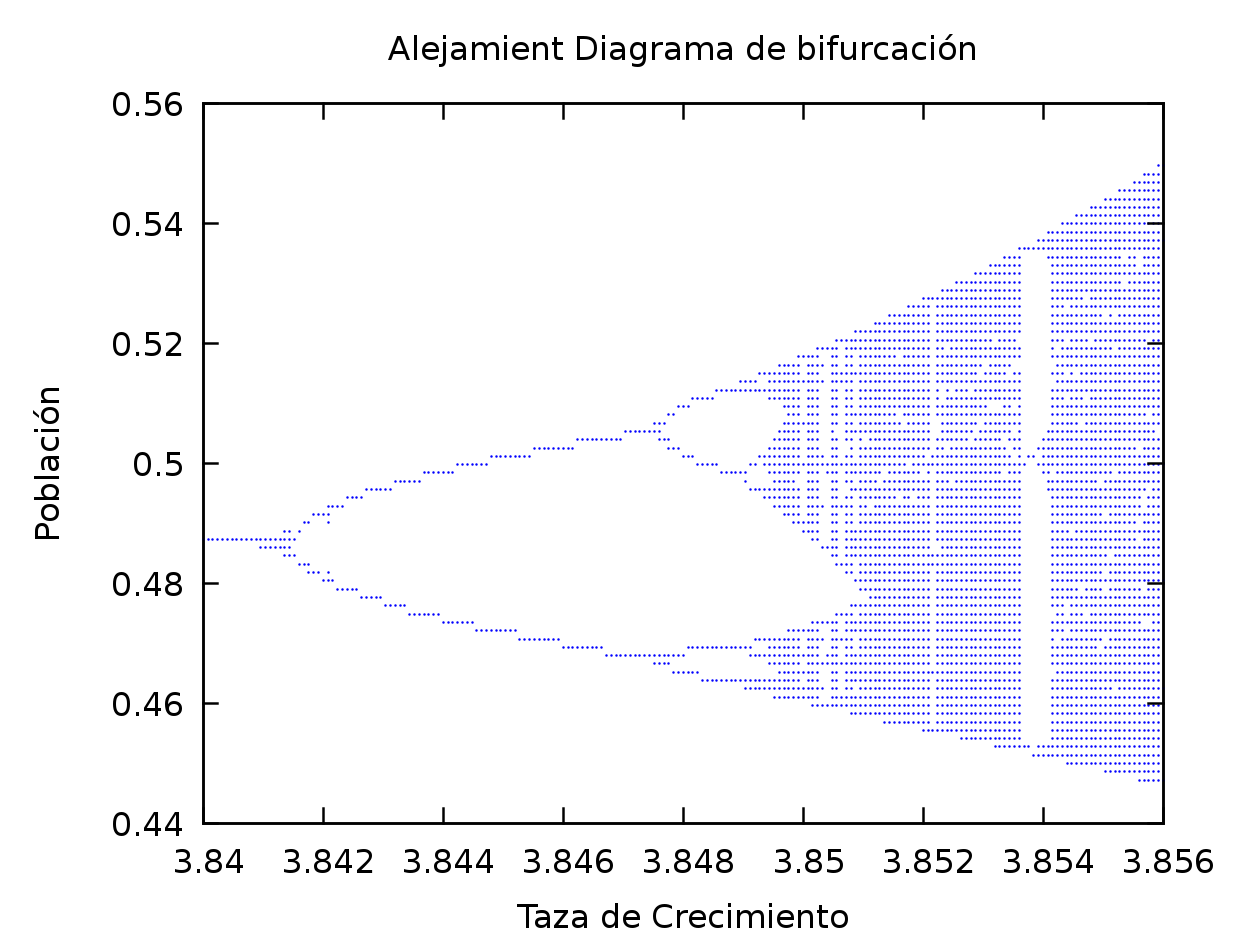
\includegraphics[height=6cm]{graf5.png}
    \centering
    \end{figure}

Debemos tener en mente que nuestro nuestro modelo sigue una simple regla determinista, por ende, si sabemos un valor de población de alguna generación en específico, podremos saber con facilidad el valor de la siguiente generación.

	\begin{center}
    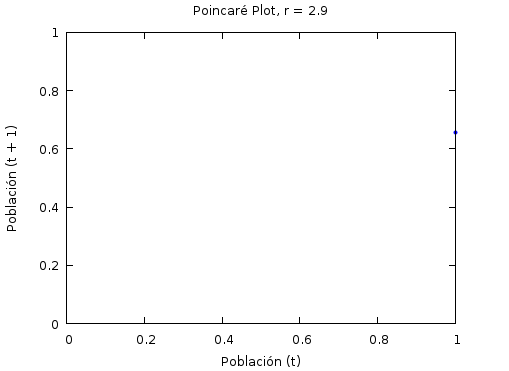
\includegraphics[height=6cm]{graf6.png}
    \end{center}
    \begin{center}
    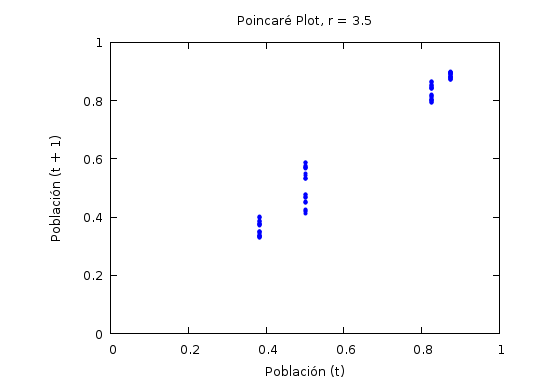
\includegraphics[height=6cm]{graf7.png}
    \end{center}

Cuando las bifurcaciones con periodo de duplicación tienden al caos, su gráfica toma forma de una parábola establecida por parámetros con tasa de crecimiento entre 3. y 4.0. Estos parámetros son mejor conocidos como el \textit{régimen caótico}, y son el rango de parámetros en los cuales el mapeo logístico se comporta de manera caótica. Cada tasa de crecimiento forma su propia curva, pero sus parábolas nunca se cruzan debido a su geometría fractal y a su naturaleza determinística obtenida de la ecuación lógica. Se puede decir que se encontró un atractor extraño cuando un sistema está extrañamente restringido pero nunca se establece en un punto fijo y su valor no sé repite.
	\begin{center}
    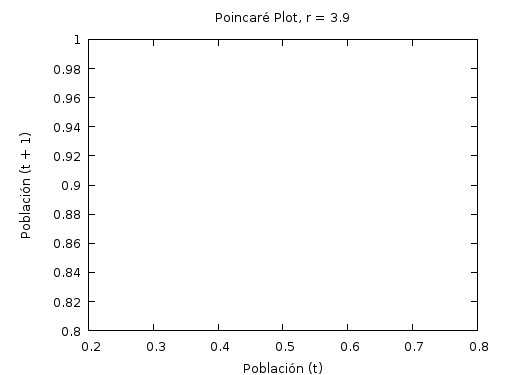
\includegraphics[height=6cm]{graf8.png}
    \end{center}
    \begin{center}
    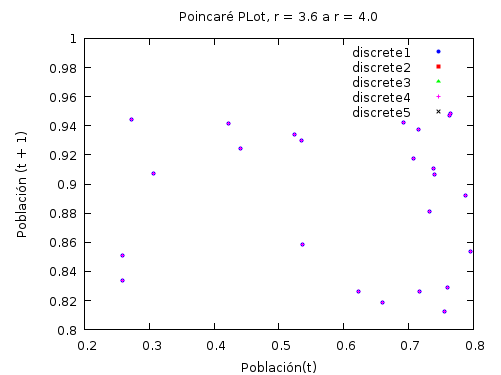
\includegraphics[height=6cm]{graf9.png}
    \end{center}
    
\section{Caos vs Aleatoriedad}
Los diagramas de fase son útiles para revelar atractores extraños en una serie de datos con tiempo al empotrar datos de una dimensión en un estado de datos de dos o tres dimensiones. Un estado de espacios es una espacio imaginario que usa un sistema de variables como sus dimensiones, cada punto en ese espacio teniendo un conjunto de valores variables. El diagrama de fase es de gran ayuda ya que muchas veces puede ser difícil el distinguir si los valores están siendo aleatorios o caóticos cuando no se tiene un buen entendimiento sobre su dinámica subyacente. Por ejemplo,

	\begin{figure}[h!]
    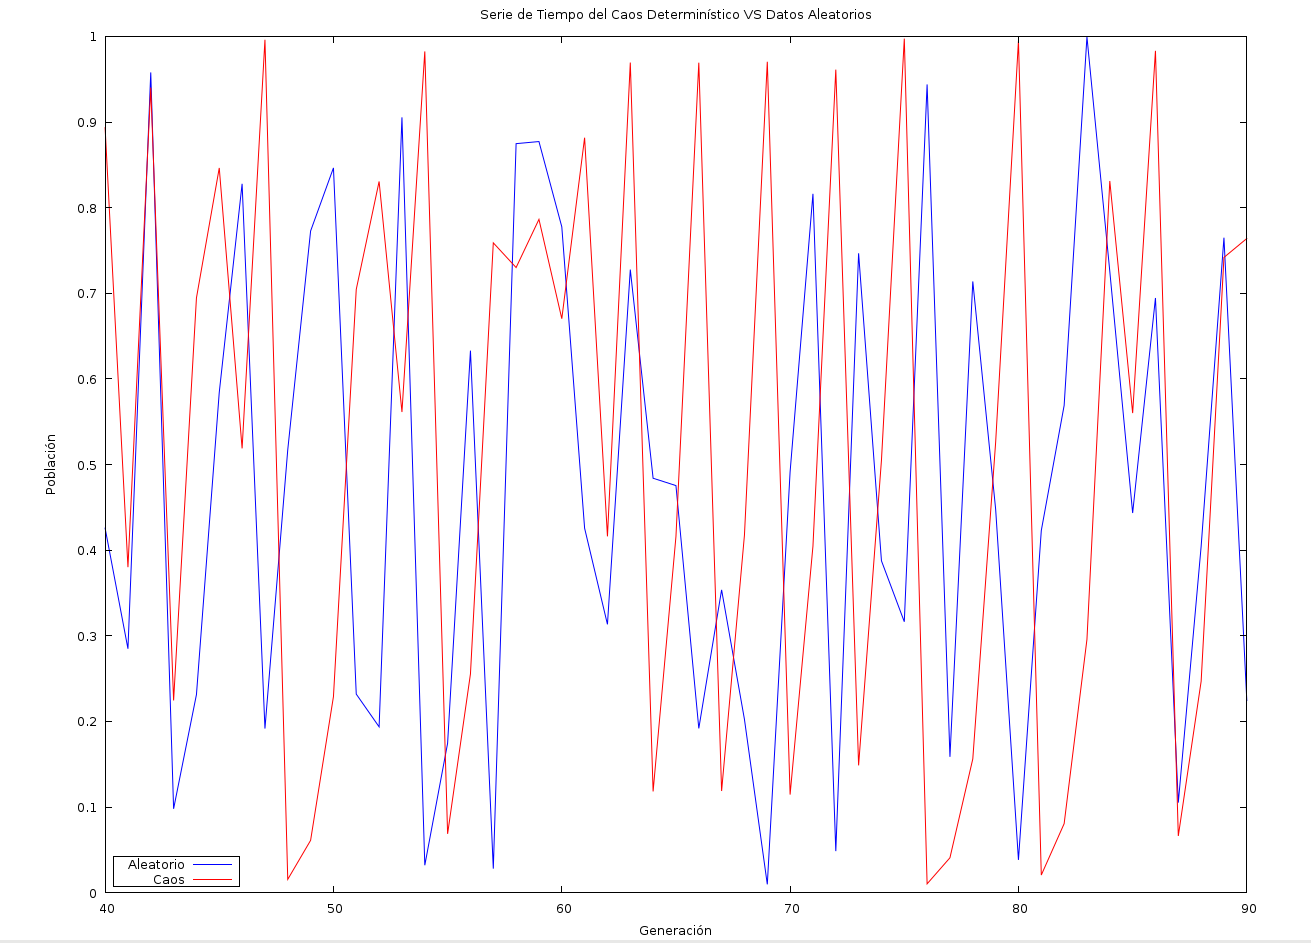
\includegraphics[height=6cm]{graf10.png}
    \centering
    \end{figure}

aquí ambas líneas parecen saltar de manera aleatoria, pero mientras la línea azul es verdaderamente aleatoria, la línea roja es caos determinístico.

Si movemos las gráfica roja a un plano de tres dimensiones y rotamos el eje, nos daríamos cuenta que esta se encuentra apretada por su atractor extraño, mientras que la gráfica azul solo mostraría ruido.	Lo mismo ocurriría si se crearan diagramas de fase para las parábolas creadas en la sección anterior.

	\begin{figure}[h!]
    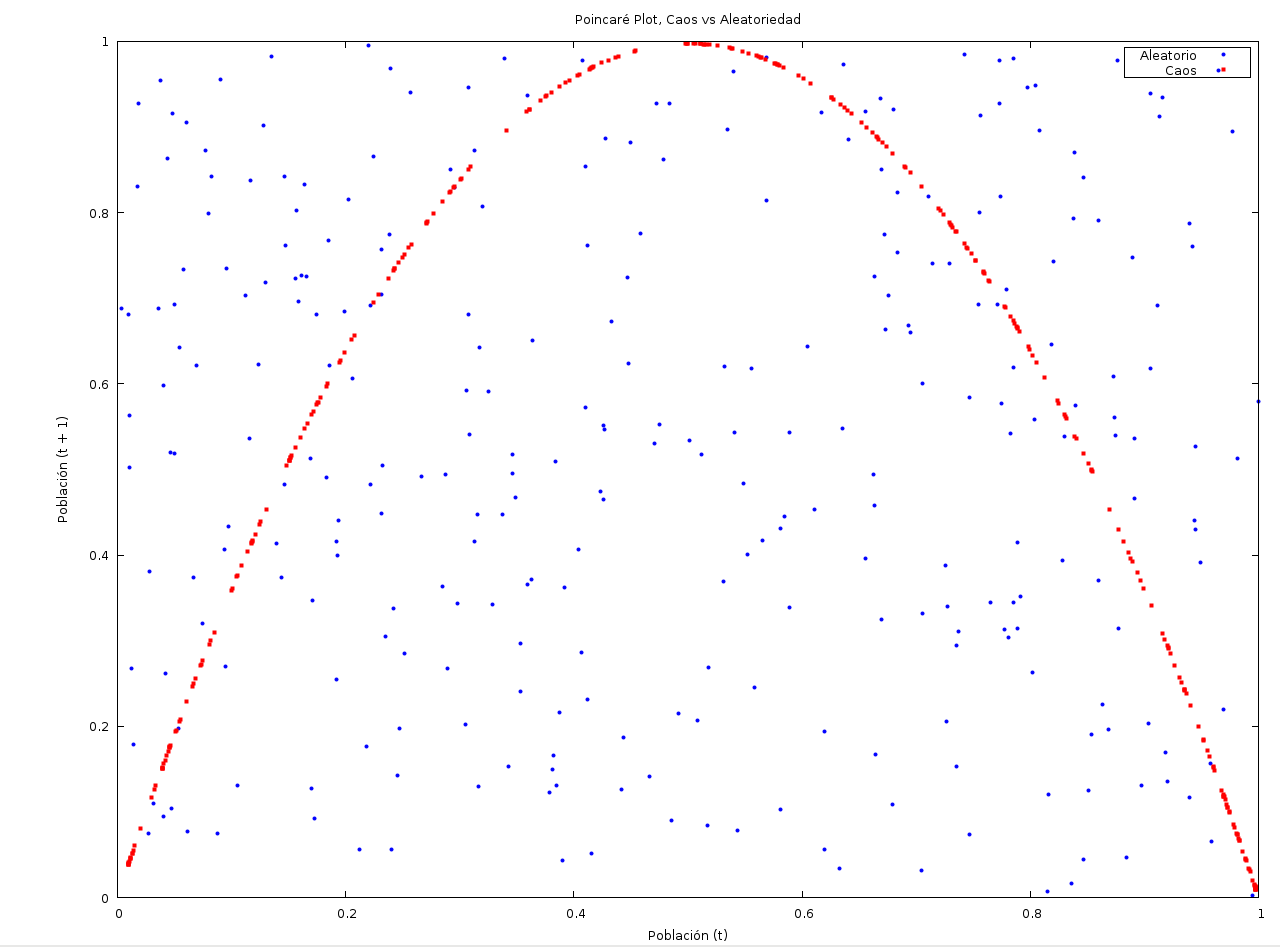
\includegraphics[height=6cm]{graf11.png}
    \centering
    \end{figure}

\section{El Efecto Mariposa}
Los sistemas caóticos son caracterizados por tener una dependencia extremadamente sensible a sus condiciones iniciales. Con un atractor extraño, puntos cercanos divergen conforme pasa el tiempo, lo cual hace un modelaje y predicción del mundo real difícil, al tener que medir los parámetros con una precisión impecable. De lo contrario, los pequeños errores en la medición, o realizar algún tipo de redondeo, hará que se tenga un sistema completamente distinto al esperado.

	\begin{figure}[h!]
    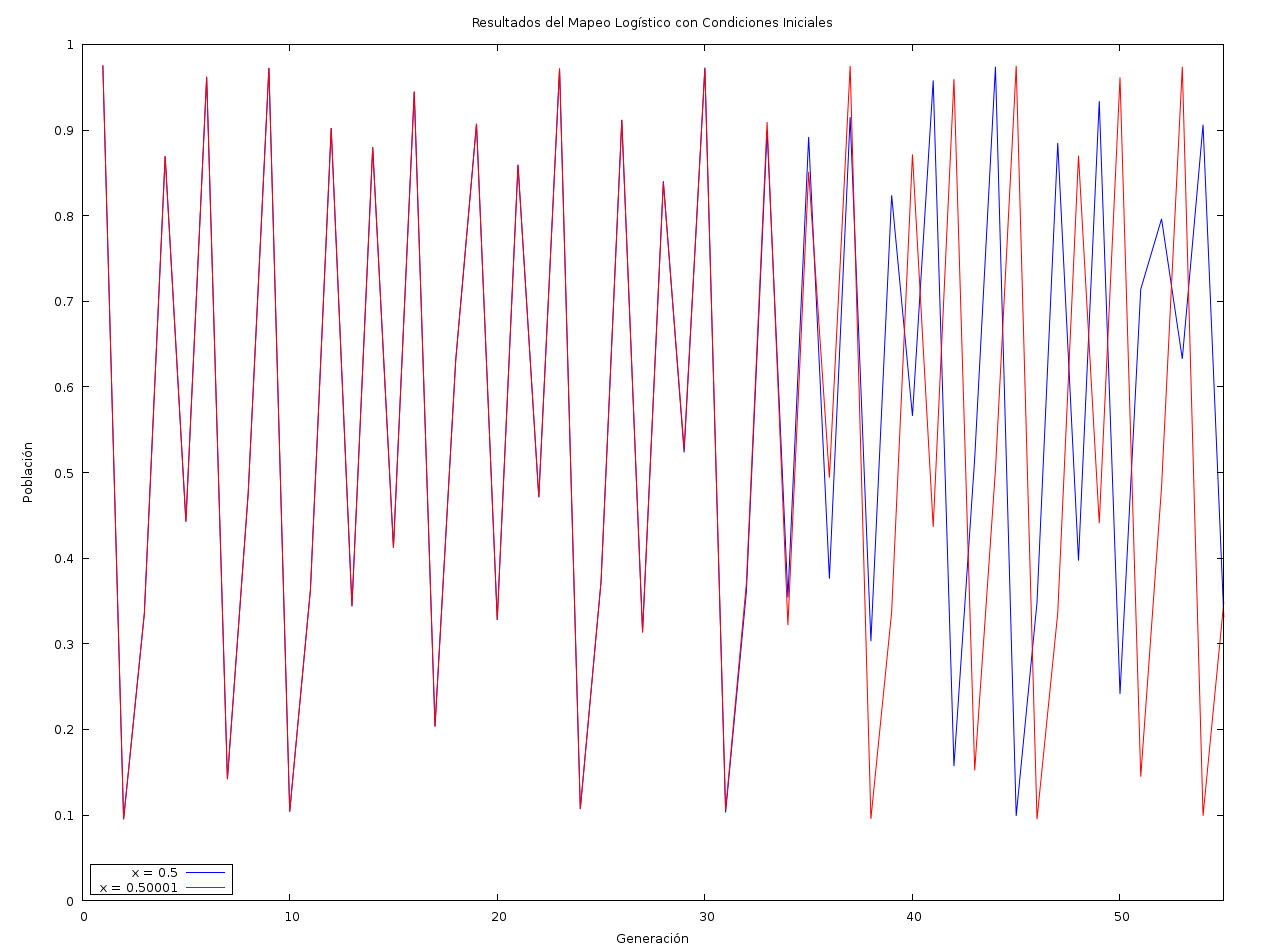
\includegraphics[height=6cm]{graf12.png}
    \centering
    \end{figure}

Tomemos como ejemplo dos gráficas que tengan valores muy similares en sus poblaciones iniciales, una iniciando en 0.5 y la otra en 0.50001. Mientras que sus resultados parecerán idénticos, después de las primeras 30 generaciones los datos empezaran a divergir hasta en punto que cuando ambas alcanzan 40 generaciones no tendrán nada en común. Si se hubiesen empezado a observar los sistemas desde la generación 50, no se tendría evidencia para decir que eran idénticos en algún punto.

Con el caos, el pasado se pierde y la predicción del futuro es tan precisa como las mediciones que realizas de ellas. En el mundo real las mediciones nunca son infinitamente precisas, por lo que al siempre tener cierto margen de error, no se puede predecir el futuro si se dan periodos de tiempo lo suficientemente largos. A este fenómeno se le denomina el \textit{Efecto Mariposa}, haciendo referencia de como pequeños eventos alteran de manera irreversible el futuro del Universo, justo como se presentó en el ejemplo de anterior.

\section{Las Implicaciones del Caos}
El caos indica fundamentalmente que existen limites en el conocimiento y predicción, encontrando modelos caóticos en el ritmo cardíaco, planeación urbana e incluso ciencias sociales. 

Durante los noventas, la teoría de la complejidad creció como rama de la teoría del caos, siendo está una manera analítica de interpretar los sistemas sociales. Aunque toma base de la teoría del caos, la teoría de la complejidad observa sistemas enormes y abiertos con muchas interacciones, ya que esta teoría logra retener algo de sus condiciones iniciales y estados previos, siendo impredecibles de una manera distinta al caos.

\section{Conclusión}
El caos determinístico es fenómeno complejo que puede verse representado en los lugares más inesperados, como en el planeamiento urbano o ritmo cardíaco. Es uno de los sistemas más difíciles de medir, ya que la más ligera diferencia en su condición inicial podría obtener un sistema completamente diferente al que se busca. Aunque a primera vista parecen datos aleatorios, el caos determinístico adquiere una forma específica cuando se gráfica en tres dimensiones.

\end{document}
